\chapter{H$_{2}$O in an external electric dc field}
\label{cha:dc_h2o}

% H2O in strong dc fields
% effective potential
% outline of the chapter

The stark resonance parameters, which characterize the shift of the
molecular energy levels under an external dc field, are fundamental in
the study of the strong dc field ionization of molecular orbitals
(\textsc{mo}s). In the case of the water molecule, the multicentre
nature of the combined Coulomb interactions and, consequently, the
additional degrees of freedom, make the strong dc field ionization of
H$_{2}$O an attractive and challenging problem from the point of view
of a theoretical description as well as experimentally. Complex
variable techniques, such as an exterior complex
scaling~\cite{Simon_1979,Scrinzi_2010} and complex-absorbing
potentiasl~\cite{RissMeyer_1993,Krause_2014}, have been implemented in
order to address the problem of molecular static-field ionization and
compute the induced Stark resonances.

The dc Stark problem for the H$_{2}$O valence orbitals is addressed in
this chapter by the implementation of a modified exterior complex
scaling approach that allows to study the ionization of the molecular
orbitals of H$_{2}$O under a strong dc field. The construction of an
effective potential, which reflects the indivual properties of the
orbitals, is crucial in this analysis. In Sec.~\ref{ch:h2o_structure},
we formulate the problem with emphasis on the representation of the
molecular orbitals. The exterior complex scaling formalism is
introduced in Secs.~\ref{ch:1b1_1b2} and~\ref{ch:3a1} as a crucial
step in finding a numerical solution to a spherically symmetric
problem, in the case of the $1b_{1}$ and $1b_{2}$ orbitals, and the
problem of a non-central effective potential, in the case of the
$3a_{1}$ orbital. The Stark resonance parameters are then presented in
Sec.~\ref{ch:stark_params}, in which the symmetry properties of the
orbitals are considered independently. The analysis presented in this
chapter compiles that of~\cite{sarias_2016,sarias_2017}.


\section{Molecular orbital representation of H$_{2}$O}
\label{ch:h2o_structure}
% Formulation of the Problem

The starting point for this study is the Hartree-Fock (\textsc{hf})
calculation of the H$_{2}$O molecular states using a single-center
Slater orbital
basis~\cite{Moccia_1964,Moccia_JCP_2164,Moccia_JCP_2176}, applied to
collision studies~\cite{Montanari_2013} and compared to experimental
electron spectroscopy~\cite{Hafied_2007}. Other elaborate descriptions
of the molecular structure of H$_{2}$O, formulated within the
independent-electron approximation by the self-consistent field
(\textsc{scf}) or variational Hartree-Fock method with multicentre
Slater orbitals in which the pioneering work of Ellison and
Shull~\cite{EllisonShullh2o_1955} is revised, are reference for
describing the electronic structure of diatomic molecules by means of
an expansion of Slater
orbitals~\cite{Pitzer_1968,Pitzer_1970}. However, the direct
application of these multicentre orbitals for strong-field studies
implies significant computational and methodological challenges.

The present work is intended to study the valence molecular orbitals
of H$_{2}$O, $1b_{1}$, $1b_{2}$ and $3a_{1}$. The wavefunctions for
the $1b_{1}$ and $1b_{2}$ molecular orbitals, which correspond to the
$2p_{x}$ and $2p_{y}$ oxygen orbitals, are dominated by a single
angular mometum symmetry. The $3a_{1}$ \textsc{mo}, on the other hand,
consists mainly of the oxygen $2s$ and $2p_{z}$ and the hydrogen $1s$
atomic orbitals.

The general expression for the basis functions, introduced as a set of
single-center
wavefunctions~\cite{Moccia_1964,Moccia_JCP_2164,Moccia_JCP_2176}, is
defined as a Slater-type orbital (\textsc{sto}),
%
\begin{eqnarray}
  \begin{split}
 f_{n, l, m}(\zeta,r,\theta,\phi) & = & \sqrt{\frac{(2\zeta)^{2n+1}}{(2n)!}}
 r^{n-1} \exp(-\zeta r) S_{l, m}(\theta,\phi),
 \end{split}
\label{eq:sto}
\end{eqnarray}
%
where the angular part $S_{l,m}(\theta,\phi)$ represents real
spherical harmonics. The expansion coefficients and nonlinear
coeficients $\{\zeta_{i}\}$, determined by the Roothaan's
self-consistent-field method~\cite{Moccia_1964,Roothaan_1951}, are
used to construct a reduced form of the radial functions that describe
all the molecular orbitals. More specifically, we are interested in
using a reduced \textsc{sto} expansion to construct an effective
pontential that describes the response of the H$_{2}$O valence
orbitals when applying an electric dc field along the symmetry axis
(i.e., the $z-$axis).

Based on their symmetry properties, independent descriptions of the
valence molecular orbitals of H$_{2}$O are constructed. The dominant
components of the $1b_{1}$ and $1b_{2}$ orbitals, namely the $np_{x}$
and $np_{y}$ parts, are used to derive spherically symmetric effective
orbital-dependent potentials~\cite{sarias_2016}. While a similar
procedure is implemented for the $3a_{1}$ orbital, i.e., retaining the
$np_{z}$ parts of the \textsc{mo}, the strong asymmetry introduced by
the two protons located in the $y-z$ plane leading to significant
admixtures of $s-$type Slater orbitals in the Moccia
\textsc{sto}s~\cite{Moccia_1964} would have been ignored with a
spherically symmetric potential. Hence, for the dc ionization problem
of the $3a_{1}$ \textsc{mo}, \textsc{sto}s of type $2s$ and $2p_{z}$
are incorporated in the analysis.


% representation of the orbitals, fig.1 in the papers (also fig.2 of
% the jphysb), with related comments

\section{$1b_{1}$ and $1b_{2}$ molecular orbitals}
\label{ch:1b1_1b2}

The Schr\"{o}dinger equation for the bound-state problem of a
molecular orbital within an effective potential $V_{\mathrm{eff}}(r)$
is expressed in shperical polar coordinates as
%
%sch. eq.
%


Figure~\ref{fig:h2o_1b1_1b2} shows a scheme of the geometry of the
system, where the orientation of the $1b_{1}$ and $1b_{2}$
\textsc{mo}s is represented with respect to the plane where the
protons are located. The direction of the applied electric field along
$\hat{z}$ is included as well.

\begin{figure}
  \centering
  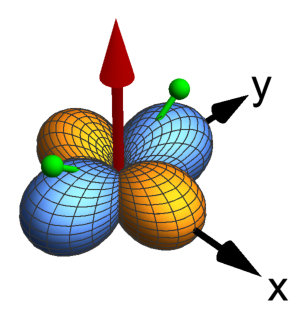
\includegraphics[width=0.25\textwidth]{figures/ch_H2O/orbitals.eps}
  \caption{Schematic display of the $1b_{1}\approx 2p_{x}$ (shown in
    yellow along the $x$ axis) and $1b_{2}\approx 2p_{y}$ (shown in
    blue along the $y$ axis) molecular orbitals. Also indicated (in
    green on the $y-z$ plane) is the orientation of the protons. The
    $z$ axis (in red) is the direction of the external electric field
    of strength $F_{0}$.}
  \label{fig:h2o_1b1_1b2}
\end{figure}

\subsection{\textsc{pde} approach in spherical polar coordinates}

\section{$3a_{1}$ molecular orbital}
\label{ch:3a1}
\subsection{Interpolation and Latter correction of the
  non-spherical effective potential}


%\section{Partial differential equation approach to the problem}
%\label{ch:h2o_pde}

%\subsection{Exterior complex scaling}
%\label{ch:h2o_ecs}

\section{Stark resonance parameters}
\label{ch:stark_params}
\subsection{$1b_{1}$ and $1b_{2}$ molecular orbitals}
\subsection{$3a_{1}$ molecular orbital}

%%% Local Variables:
%%% mode: latex
%%% TeX-master: "thesis"
%%% End:
